\chapter{Теория}
\section{Структурная схема модели}

В процессе взаимодействия клиентов и центра возможны:
\begin{itemize}
	\item режим нормального обслуживания (когда клиент выбирает одного из свободных операторов, но предпочитает того, у которого меньше номер);
	\item режим отказа.
\end{itemize}

Структурная схема модели представленна на рисунке \ref{s2}.

\begin{figure}[h]
	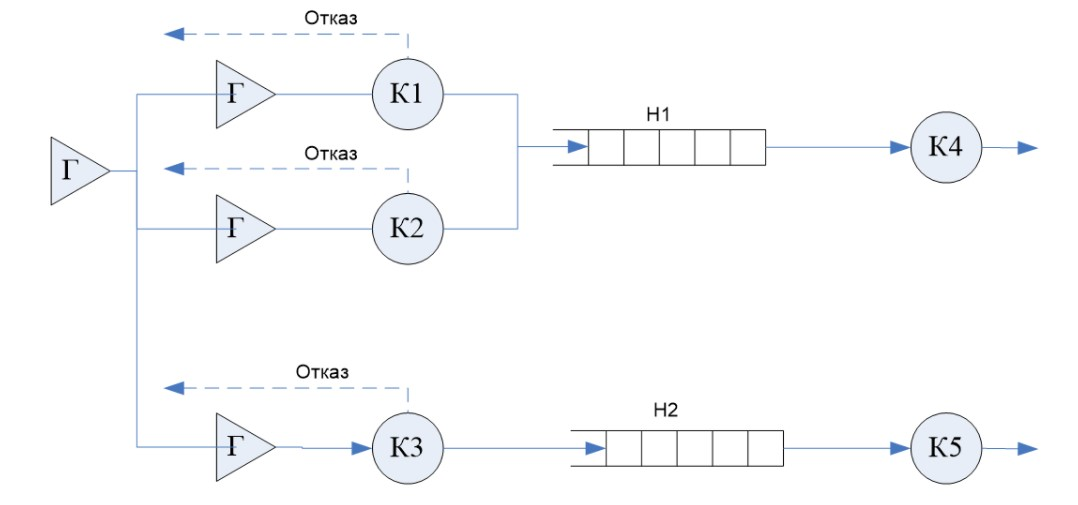
\includegraphics[width=1\linewidth]{inc/img/schema2.jpg}
	\caption{Структурная схема модели}
	\label{s2}
\end{figure}

Согласно условию время обработки заявки оператором подчиняется закону равномерного распределения, а компьютер выполняет каждую обработку за фиксированное время.

Эндогенные переменные -- время обработки заданий $i$-ым оператором ($i = \overline{0;2}$) и время решения задания на $j$-ом компьютере ($j = \overline{0;1}$).

Экзогенные переменные -- $n_0 =$ числу обслуженных клиентов, $n_1 =$ числу клиентов получивших отказ.

Уравнения модели: вероятность отказа $= n_1/(n_0+n_1)$

За единицу дискретного времени выбрана 0.01 минуты.
